\documentclass{article}
\usepackage[utf8]{inputenc}
\usepackage{graphicx}
\graphicspath{ {images/} }
\usepackage{amsmath}
\usepackage{amssymb}
\DeclareUnicodeCharacter{2212}{-}
\title{Estado del arte en circuitos caóticos}
\author{asd}
\date{Noviembre 2022}

\begin{document}

\maketitle
\section{tipos de circuitos caóticos}
Dimensión 
1D RL-Diode
2D
3D Chua, Colppits
4D Saito

2.- Autónomos y no autónomos
\section{Circuito de Saito}

    Los fenómenos caóticos en los circuitos eléctricos se han estudiado con gran interés. En particular, los circuitos autónomos tridimensionales y los circuitos no autónomos bidimensionales han sido bien investigados y se han publicado algunos resultados analíticos excelentes (l-7). También se han publicado recientemente algunos resultados experimentales de circuitos caóticos autónomos de cuatro dimensiones (8-9). Creemos que el análisis de los circuitos de mayor dimensión es muy importante para desarrollar la teoría de los circuitos caóticos, y por lo tanto, deben ser estudiados con más detalle. La parte 1 da un circuito autónomo simple de cuatro dimensiones que realiza el hipercaos, un caos de dimensión superior introducido por Rossler (10). El hipercaos suele definirse como un atractor caótico con más de un exponente de Lyapunov positivo. No puede observarse en los circuitos autónomos tridimensionales porque un exponente de Lyapunov es siempre cero y debe haber al menos un exponente negativo para que sea un atractor (8). La Fig. 1 muestra el circuito objetivo. 
    \begin{figure}[h]
        \centering
        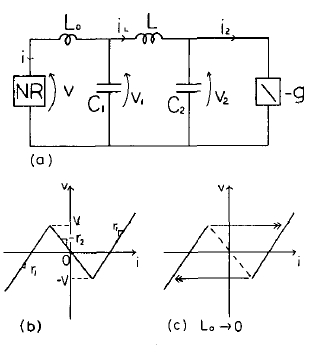
\includegraphics[width=0.5\textwidth]{Saito/fig. 1 Saito.png}
        \caption{Hyperchaos generator.}
        \label{fig1:saito}
    \end{figure}
    En este circuito, - g es un conductor lineal negativo caracterizado por i, = - gv, y NR es una resistencia no lineal controlada por la corriente caracterizada por una función lineal a trozos de la Fig. l(b):
    \begin{figure}[h]
        \centering
        \includegraphics[width=0.5\textwidth]{Saito/ec1 saito.png}
        \caption{Ec.1}
        \label{fig ec1:saito}
    \end{figure}
    Algunos hechos experimentales muestran que NR funciona como una resistencia de histéresis de la Fig. l(c) si el pequeño inductor La está en cortocircuito. NR y - g son fácilmente realizables mediante los circuitos de la Fig. 2. Para simplificar los argumentos, se supone que el amplificador óptico es lineal y que el diodo zener es ideal. La dinámica del circuito se describe mediante la ecuación básica: 
    \begin{figure}[h]
        \centering
        \includegraphics[width=0.5\textwidth]{Saito/ec2 saito.png}
        \caption{Ec. 2}
        \label{fig ec2:saito}
    \end{figure}
    Obsérvese que al principio, (2) se transforma en una ecuación de forma canónica que incluye un pequeño parámetro c (cc L,). Dejando que E tienda a cero, la ecuación se simplifica en un sistema restringido, y se puede derivar rigurosamente de ella un mapa de Poincare bidimensional. Los experimentos de laboratorio indican bifurcaciones desde soluciones periódicas a cuasi-periódicas (el llamado toroide) y luego a diferentes tipos de soluciones caóticas. Estos datos se reproducen mediante soluciones numéricas del sistema restringido. El mapa de Poincare y sus exponentes de Lyapunov verifican la generación de hipercaos y fenómenos relacionados. 
    \begin{figure}[h]
        \centering
        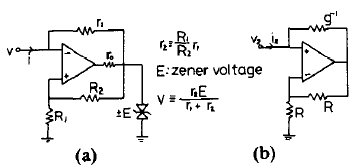
\includegraphics{Saito/fig. 2 saito.png}
        \caption{Realization of NR and -g.}
        \label{fig2:saito}
    \end{figure}

\section{circuito de Chua}

    Entre los sistemas caóticos más típicos y de fácil acceso figuran los circuitos electrónicos. \cite{kennedy1993three} menciona que deben satisfacerse tres criterios relacionados con los elementos que deben tener los circuitos: 
    
    (i) Al menos un elemento no lineal.
    
    (ii) Al menos una resistencia localmente activa (resistencia negativa). 
    
    (iii) Tres o más elementos de almacenamiento de energía.

    El circuito de Chua (Fig.~\ref{fig:circuito de Chua}) cumple estos criterios y es uno de los más populares que exhibe caos, puesto que es un circuito autónomo simple capaz de mostrar comportamiento caótico; está compuesto, por una porción que presenta el comportamiento típico de un oscilador amortiguado (dos condensadores $C_1$ y $C_2$, una resistencia variable $R$ y una bobina $L$) y la otra parte que constituye el único elemento no lineal denominado diodo de Chua, $N_R$ que básicamente es una resistencia no lineal negativa o lineal por partes (piecewise linear o PWL) como se muestra en la Fig.~\ref{fig:diodo teórico}. Este elemento causante de la no linealidad actúa como la fuente de energía de todo el circuito, ya que es la responsable de la retroalimentación que lo mantiene oscilando.
    
    \begin{figure}[h!]
        \centering
        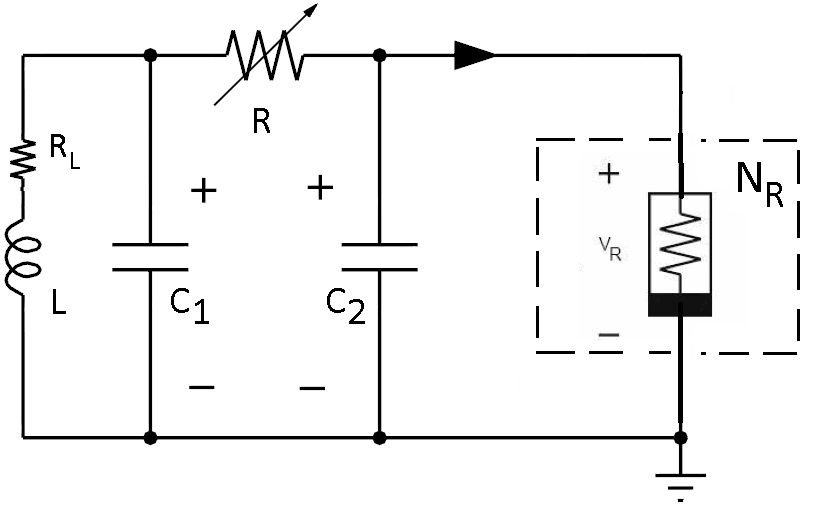
\includegraphics[width=0.8\textwidth]{Chua/circuitodechua.png}
        \caption{Circuito de Chua canónico}
        \label{fig:circuito de Chua}
    \end{figure}
    
    Escribiendo las variables dinámicas $V_{C_1}$, $V_{C_2}$ e $I_L$, junto con los voltajes de quiebre $-B_{p}$ y $+B_{p}$, como:
    %Ec. 1
    \begin{eqnarray}
        \begin{aligned}
            x & = V_{C_1}(B_p)^{-1},\\
            y & = V_{C_2}(B_p)^{-1},\\ 
            z & = RI_L(B_p)^{-1},\\ 
            \tau & = t(RC_2)^{-1}\\
        \end{aligned}
    \end{eqnarray}
    se obtiene las ecuaciones diferenciales adimen\-sio\-na\-les:
    %Ec. 2
    \begin{eqnarray}\label{Chua eq dif}
        \begin{aligned}
            \dot{x} &= \alpha(y - x - f(x)),\\
            \dot{y} &= x-y+z,\\
            \dot{z} &= -\beta y - \gamma z,
        \end{aligned}
    \end{eqnarray}
    con los parámetros:
    %Ec. 3
    \begin{eqnarray}\label{alfa beta gamma}
        \begin{aligned}
            \alpha & = C_{2} C_{3}^{-1},\\
            \beta & = R^{2} C_2 L^{-1}, \\
            \gamma & = R_{L} RC_{2} L^{-1},
        \end{aligned}
    \end{eqnarray}
    donde $R_L$ representa la resistencia interna del inductor $L$ en la Fig.~\ref{fig:circuito de Chua}. A esta configuración se la conoce como circuito de Chua canónico ($\mathfrak{C}^2$), en el sentido de que puede exhibir todos los posibles comportamientos dinámicos asociados con cualquier campo vector continuo, lineal por partes (PWL) y simétrico de tres regiones. En el caso de no con\-si\-de\-rar la resistencia $R_L$, el valor de $\gamma$ es nulo y el circuito de Chua ($\mathfrak{C}^1$) se convierte en el caso simple/ideal.
    \begin{figure}[h!]
        \centering
        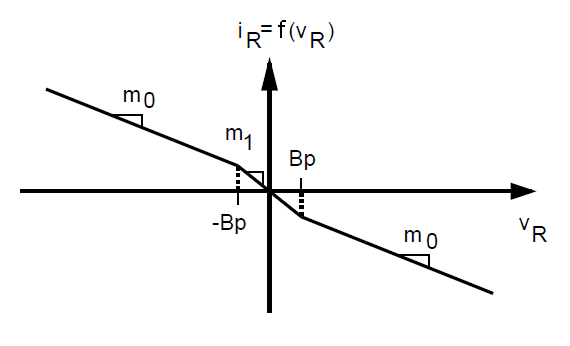
\includegraphics[width=0.8\textwidth]{Chua/DiodoChua.png}
        \caption{Característica de linealidad por partes de voltaje y corriente del diodo de Chua. $-B_{p}$ y $+B_{p}$ son los puntos de quiebre de la relación corriente-voltaje del diodo de Chua; en tanto que $m_{0}$ y $m_{1}$ son las pendientes de la región externa e interna, respectivamente (\cite{kennedy1992robust}).} 
        \label{fig:diodo teórico}
    \end{figure} 
    La función PWL que describe el comportamiento del diodo de Chua, es:
    %Ec. 4
    \begin{equation}\label{f(x) PWL}
        f(x) = m_{0}x + (1/2)(m_{1}-m_{0})(|x+B_p|-|x-B_p|),
    \end{equation}
    las pendientes $m_0$ y $m_1$ se pueden escribir como:
    %Ec. 5
    \begin{eqnarray}\label{pendientes}
        \begin{aligned}
            m_0=(-R_3^{-1} +R_4^{-1}),\\
            m_1=(-R_3^{-1} -R_6^{-1}).
        \end{aligned}
    \end{eqnarray}

\section{circuito RL-Diodo}
    En general, se dice que para observar comportamientos caóticos, es necesario que el sistema sea de tercer orden o mayor. En el caso de los circuitos autónomos, se necesita que el sistema se componga de un elemento no lineal y por lo menos tres elementos lineales que almacenen energía (inductor, resistencia, capacitor), como se ha visto con el circuito de Chua, es autónomo porque no necesita de fuentes de energía alterna ya que es el mismo circuito el que transforma la señal continua proveniente del diodo en alterna, además el diodo de Chua es la pieza clave para el comportamiento no lineal de todo el circuito. No obstante, esta regla no es definitiva puesto que puede existir caos en un sistema más sencillo compuesto por una resistencia lineal, un inductor lineal, un diodo normal y una fuente de voltaje. El circuito RL-Diodo,al contrario tiene una fuente de energía alterna, por lo que se lo denomina no autónomo, y tres elementos que bajo ciertos parámetros de frecuencia y amplitud, se generan señales aperiódicas mediante el desdoblamiento de periodo de la tensión en el diodo. Entonces, a un circuito RLC se reemplaza el condensador por un diodo normal (ver Fig.), el cual al ser un elemento no lineal, es el causante de las aperiodicidades. En este circuito se asume que el voltaje de la fuente tiene la forma $V_a = V_0\cos(\omega t)$ y cuando el voltaje es positivo, el diodo conduce y se produce una caída de voltaje $V_b = −V_f$. En el estado no conductor, el diodo se comporta como un capacitor, el cual presenta una corriente de carga y el voltaje sigue la frecuencia de la fuente. La amplitud del voltaje de fuente $\lambda=V_0$ es el parámetro de control. Esta amplitud no necesariamente es igual para cada ciclo porque cuando la corriente llega a cero, el diodo continúa conduciendo con un tiempo $\tau_r=\tau_{m}(1−e−|I_m|/I_c)$, donde $|Im|$es la corriente máxima durante ese ciclo, $\tau_mel$ tiempo máximo constante, $\tau_rel$ tiempo de recuperación e $I_{ces}$ constante. Por lo tanto, dependiendo del parámetro $V_0$, el voltaje en el diodo $V_bse$ repite con un periodo y se va desdoblando hasta llegar al caos. Como el voltaje en el diodo depende del voltaje de la fuente y éste depende también de la frecuencia $f=w/2pi$, se espera un comportamiento similar con su variación [13]. Uno de los caminos más comunes para llegar a un comportamiento caótico es el desdoblamiento de periodo en el que las bifurcaciones mediante éste fenómeno ocurren solamente con soluciones periódicas o trayectorias que bajo un punto de bifurcación tienen periodo TY bajo otro punto de bifurcación sufren un cambio ligero presentando un periodo 2T. En el espacio de fases se observaría un ciclo límite (un lazo) que bajo cierto parámetro se convertiría en un ciclo límite de segundo orden (dos lazos) y así sucesivamente los lazos continuarían desdoblándose al igual que las soluciones con un periodo $T_k = 2kT_0$ donde k= 0, ..., n. Si se observa este proceso es muy probable que el sistema llegue a ser caótico 14. Una característica del desdoblamiento de periodo es que los puntos de bifurcación (parámetros de control) $\lambda_k$ convergen geométricamente al llegar a la región caótica. Este valor llegó a ser universal por presentarse en varios sistemas caóticos y se denomina primera constante de Feigenbaum.

    \begin{figure}
        \centering
        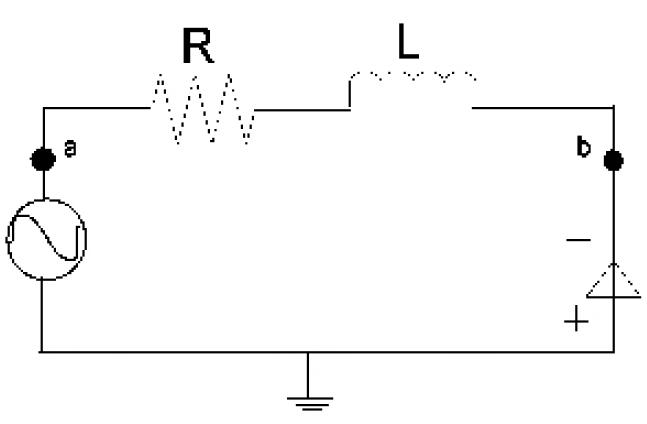
\includegraphics[width=0.5\textwidth]{RLDiodo/RLDIODO.png}
        \caption{Circuito RL-Diodo.}
        \label{fig:my_label}
    \end{figure}




%%%%%%%%%%%%%%%%%%%%%%%%%%%%%%%%%%%%%%%%%%%Sergiusss
\section{Circuito de Hartley}
La versión del circuito de \mbox{Hartley} dada por  \cite{kvarda};  consiste en un transistor bipolar $Q_1$, dos inductores $L_1$ y $L_2$ cada uno en serie con una resistencia $R_{L_1}$ y $R_{L_2}$ respectivamente, un resistor \mbox{lineal} $R_{L}$ y un capacitor lineal en paralelo  con una resistencia $R_C$, como se muestra en la Fig. 8. Las ecuaciones  que gobiernan  el sistema se muestran a continuación:

\begin{figure}
\centering
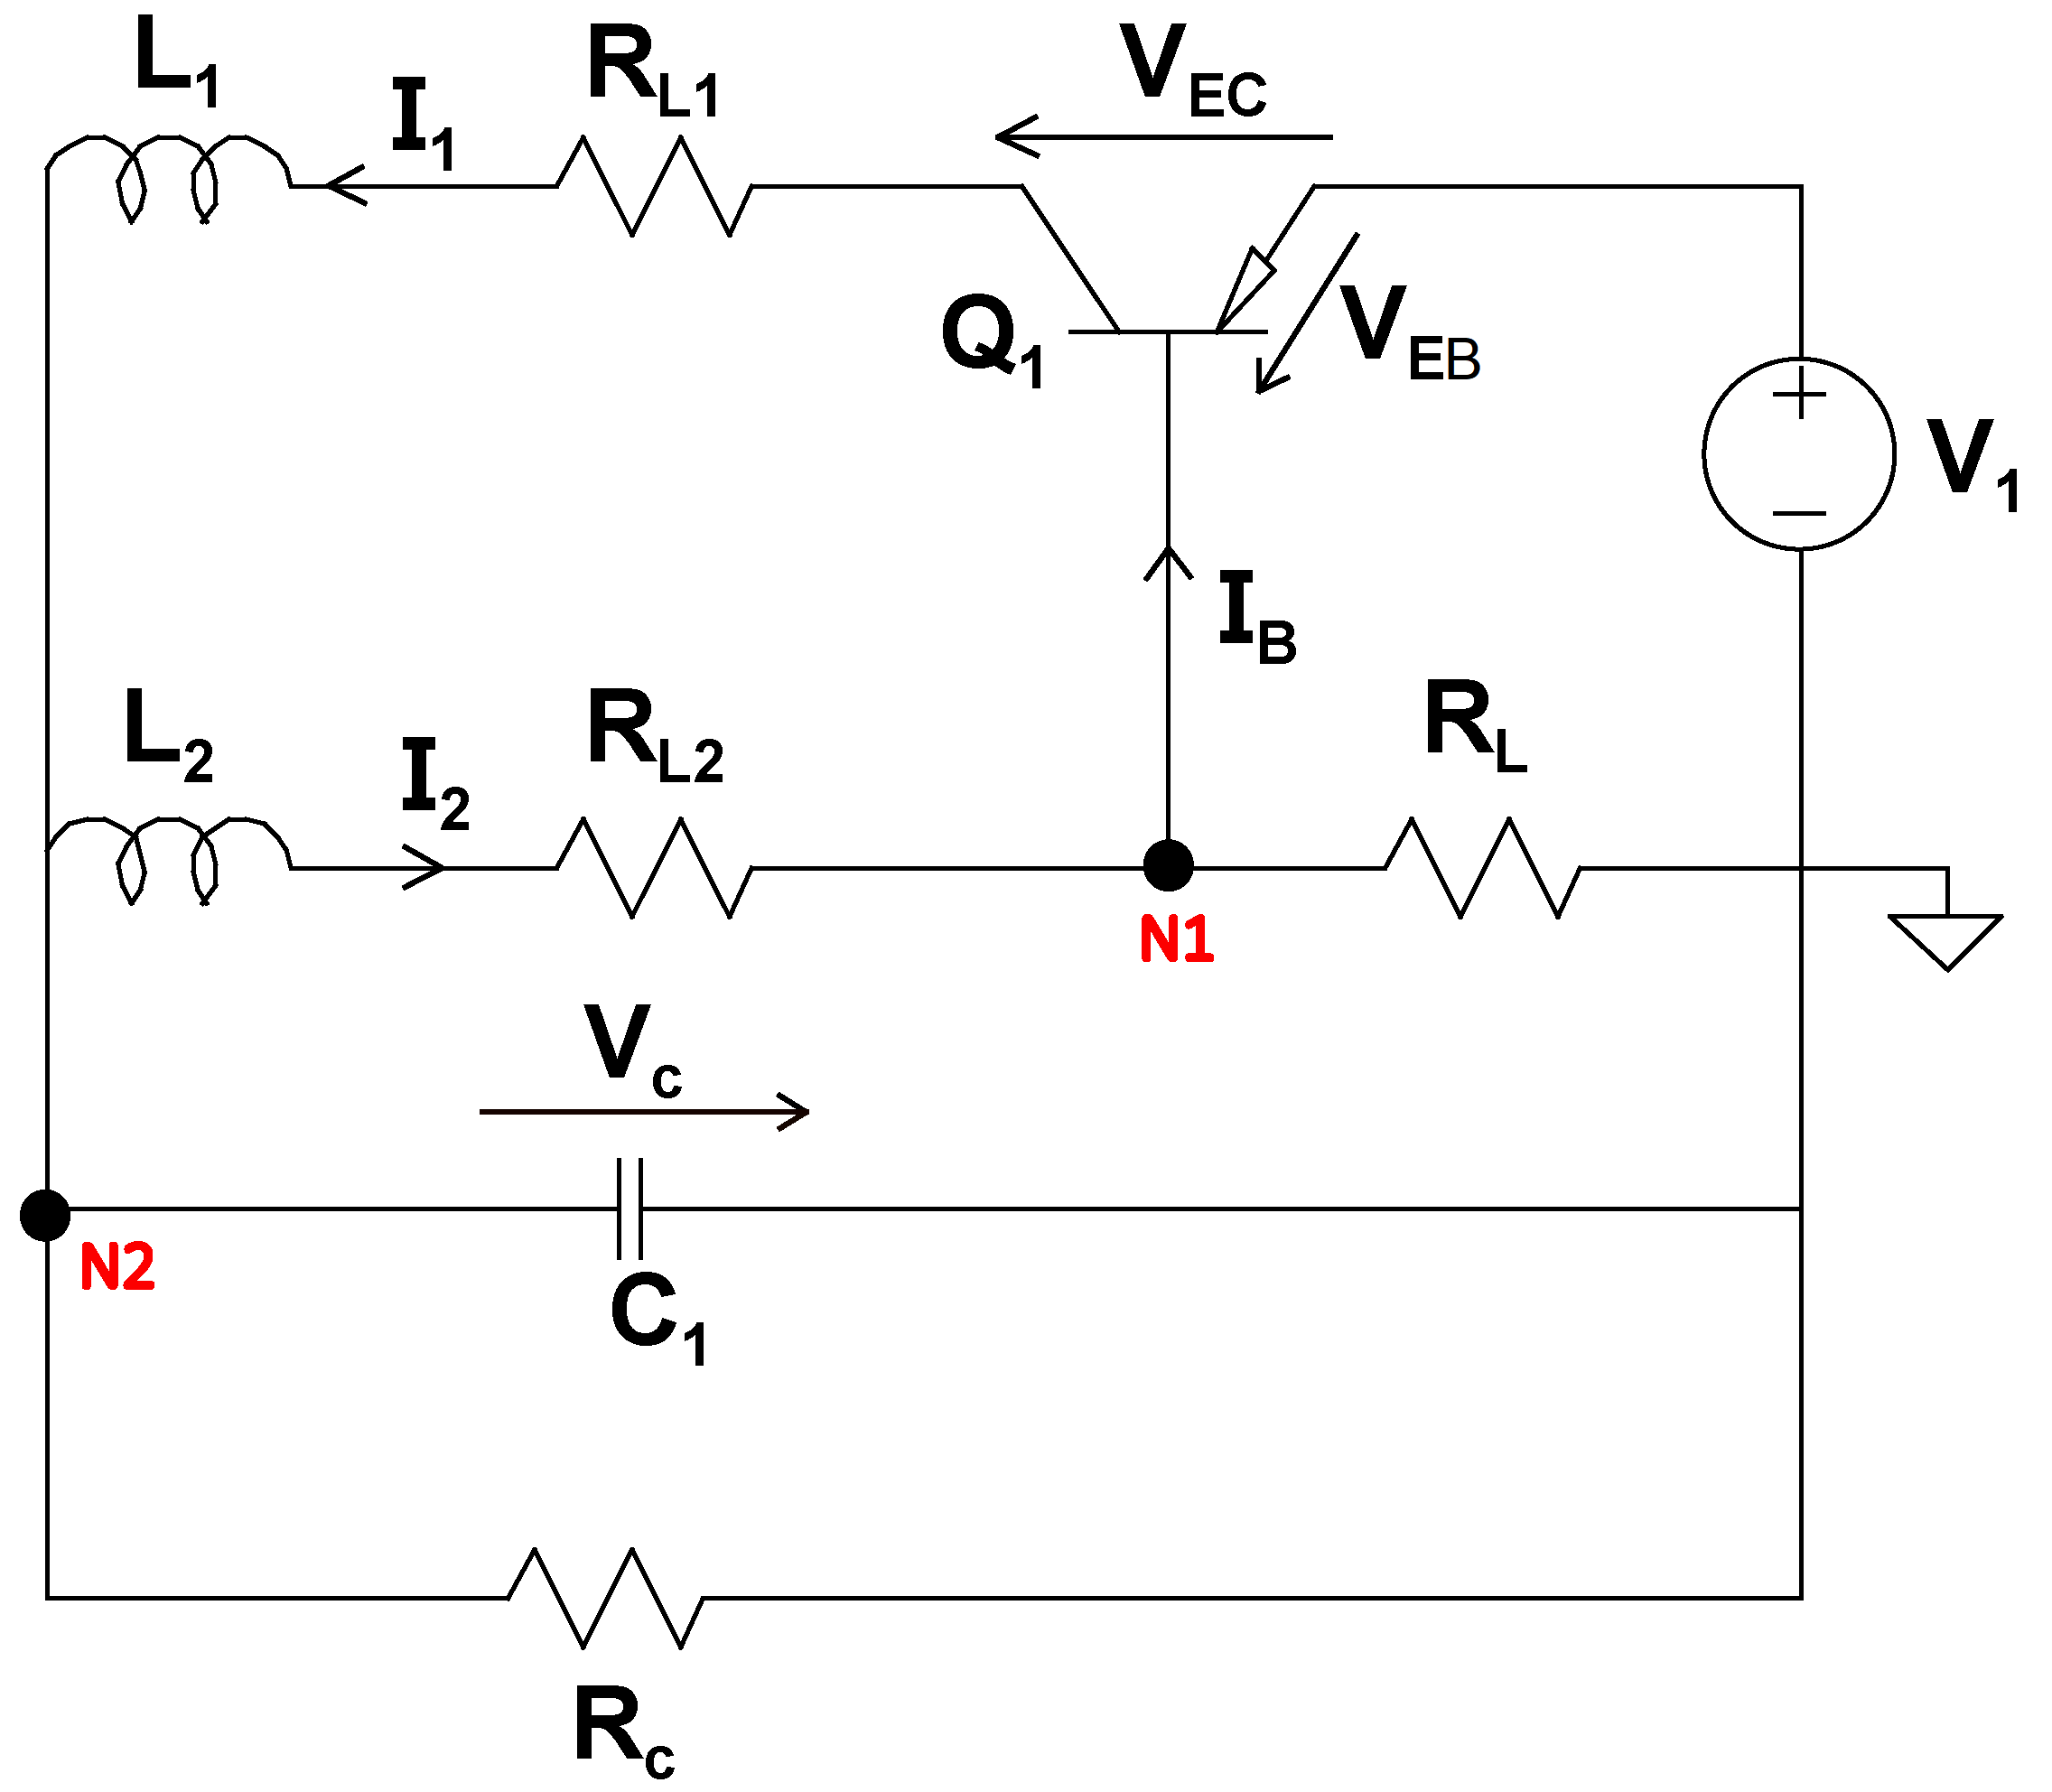
\includegraphics[scale=0.12]{Hartley/circuito hartley.png}
\caption{\label{fig2}Esquema del circuito de Hartley donde N1 y N2 son los nodos 1 y 2, puntos que se analizan en el experimento.}
\end{figure}

\begin{equation}
 \left\lbrace\begin{array}{lcc}
 
  C_{1}\frac{dV_{C}}{dt} = I_{1}-I_{2}-\frac{V_{C}}{R_{C}} \\\\  
   L_{1}\frac{dI_{1}}{dt} = V_{1}+V_{EC}-V_{C}- I_{1}R_{L_1} \\\\ 
  L_{2}\frac{dI_{2}}{dt} = V_{C}+I_{2}R_{L_2}-(I_{2}- I_{B})R_{L} \end{array}\right. 
\label{eq:one}
\end{equation}

\begin{equation}
 \left. \hspace{1.8cm} V_{EB} = V_{1}-(I_{2}-I_{B})R_{L} \right.   
  \label{eq:two}
 \end{equation}


\begin{equation}
I_{B}=\left\{ \begin{array}{ccc} 0  &  \mathrm{si}  & V_{EB}\leq V_{TH} \\ -(\frac{V_{EB}-V_{TH}}{R_{0N}})&    \mathrm{si}  &   V_{EB}>{V_{TH}} \end{array}\right. 
\end{equation}


\begin{equation}
V_{EC}=\left\lbrace\begin{array}{ccc} -k(V_{EB}-V_{TH})&  \mathrm{si}  & V_{EB}\leq  V_{TH} \\  V_{EC0}&    \mathrm{si}  &V_{EB}>{V_{TH}} \end{array}\right. 
  \label{eq:four}
\end{equation}





Las Ecs. (6) y (7) son obtenidas aplicando las leyes de Kirchhoff, en tanto las Ecs. (8) y (9) son las  que modelan el comportamiento del transistor PNP 2N3906; donde $I_B$ es la corriente de base, $V_{EC}$ es el voltaje del emisor-colector, $V_{TH}$ es el voltaje umbral del transistor, $V_{EB}$ es el voltaje entre el emisor  y la base, $V_{EC0}$ es el voltaje restante en el transistor abierto y $k$ es la pendiente de conmutación que  se define como una relación entre   $|\Delta$V$_{EC}$$|$ y $|\Delta$V$_{EB}$$|$. 

Los parámetros del circuito donde se evidenció comportamiento caótico  son:
\mbox{$V_{1}= 3.75$} V, $R_{L_1}=1.5\ \Omega$, \mbox{$R_{L_2}= 1.5\ \Omega$}, $L_{1}= 100\ \mu$H, $L_{2}= 100\ \mu$H,
\mbox{$C_{1}= 22\ n$F}, \mbox{$R_{C}= 95.5\ \Omega$}, $R_{L}= 76\ \Omega$, $B_{F}= 180$,
$k = 900$, \mbox{$V_{TH}= 0.75\  $V}, $V_{EC0}= 0.2\  $V y $R_{0N}= 100\ \Omega $.

\section{Circuito Colpitts}
Otro ejemplo de circuito caótico que utiliza un solo transistor es el oscilador de Colpitts este circuito tiene muchas configuraciones posibles debido a la combinación de inductancias capacitores y resistencias y un elemento no lineal generalmente un transistor es usado para generar formas de onda periódicas se ha demostrado que para algunos valores de parámetros comportamientos caóticos pueden ser obtenidos mostrando que es posible diseñar osciladores capaces de generas señales caóticas de alta frecuencia.Las ecuaciones del circuito caótico de Colpitts cuyo esquemático esta dado por la figura son representados por las siguientes ecuaciones de estado:
\begin{equation}
 \left\lbrace\begin{array}{lcc}
 
  C_{1}\frac{dV_{1}}{dt} = I_{L}+{\beta i_{B}} \\\\  
   C_{2}\frac{dV_{2}}{dt} =\frac{V_{ee}-V_{2}}{R_{2}} -V_{C}+ I_{L}+I_{B} \\\\ 
  L\frac{dI_{L}}{dt} = V_{cc}-V_{1}-V_{2}-R_{1}I_{L}
  \end{array}\right. 
\label{eq:one}
\end{equation}

  \begin{figure}
        \centering
        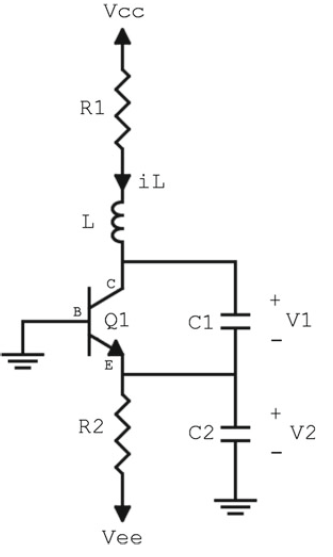
\includegraphics[width=0.5\textwidth]{Colpitts/cirucito-Colpitts.png}
        \caption{Esquema del circuito de Colpitts donde  R1 = 35$\Omega$,
R2 = 500$\Omega$, C1 = 54 nF,
C2 = 54 nF, L = 98.5μH,
2N2222 BJT transistor, Vcc =5V, Vee = −5V}
        \label{fig:my_label}
    \end{figure}

\section{Circuitos caóticos basados en componentes histeréticos}
Uno de los mecanismo para generar caos incluyen componentes hiteréticos, la topología fue introducida por Saito cuyo principio es usado para generar caos en un circuito incluyendo un dispositivo ferroeléctrico que exhibe histéresis.
El circuito eléctrico diseñado por Saito se muestra en la figura 1. este consiste en dos inductores dos capacito-res una resistencia negativa y un resistor no lineal La peculiaridad es que para pequeños avalores de Lo la resistencia no-lienal opera como un elemento con histéresis .El segmento interno de pendiente −r1 no está interesado en la trayectoria caótica que solo pasa a través de los segmentos externos que tienen una pendiente igual a r1.
En el límite del pequeño L0 la trayectoria salta de un segmento exterior al otro como se representa esquemáticamente en la figura 1.11. Esto genera un mecanismo de conmutación entre dos regiones donde la dinámica está regulada por ecuaciones lineales. Cuando la conmutación se vuelve irregular, se obtiene un comportamiento caótico. De hecho, el circuito exhibe bifurcaciones de órbitas periódicas a toros y luego a atractores caóticos y es
también capaz de generar hipercaos, es decir, un régimen en el que dos exponentes de Lyapunov son positivos.

\begin{equation}
 \left\lbrace\begin{array}{lcc}
 
  C_{1}\frac{dV_{1}}{dt} =- I_{L}+I_{R} \\\\  
   C_{2}\frac{dV_{2}}{dt} =-G_{v2}+ I_{2} \\\\ 
  L\frac{dI_{L}}{dt} = V_{1}-V_{2}\\\\
  L_{0}\frac{dI_{R}}{dt} = V_{1}-f(i_{R})
  \end{array}\right. 
\label{eq:one}
\end{equation}
  \begin{figure}
        \centering
        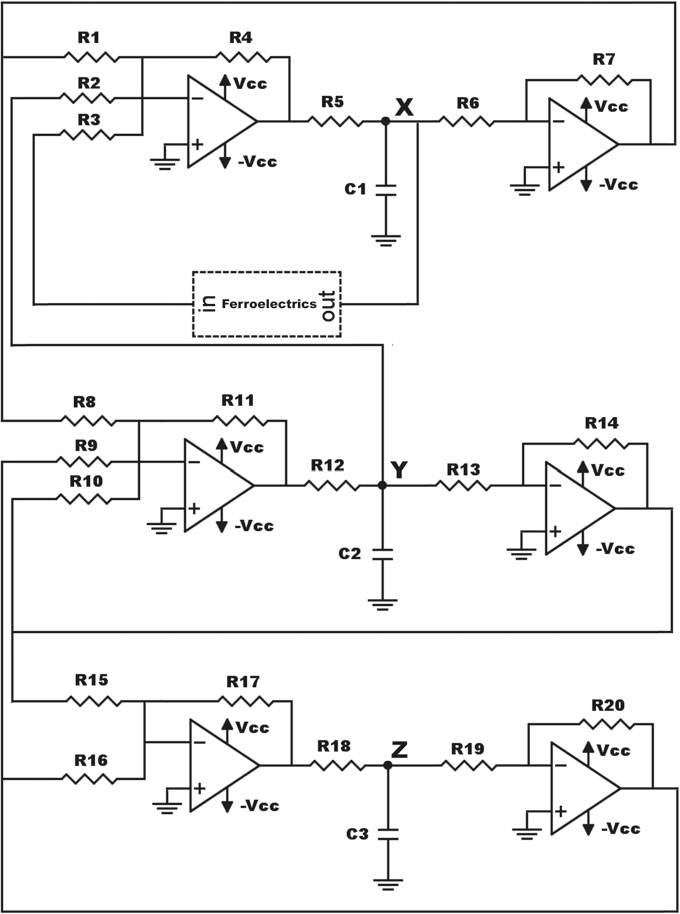
\includegraphics[width=0.8\textwidth]{circuitoH/H.png}
        \caption{Esquema del circuito caótico incluyendo un componente ferroeléctrico.
}
        \label{fig:my_label}
    \end{figure}

\section{Circuito Jerk}
Un simple circuito de Jerk nos permite estudiar la dinámica caótica en términos de variables teóricas y su equivalente salida experimental el diseño de este circuito presenta comportamiento caótico dependiendo de valor de un solo parámetro La variación de A permite observar la ocurrencia de la trayectoria de firk y su evolución al caos facilitando el entendimiento del caos y su fácil implementación experimental el circuito.cabe aclarar que el circuito de Jerk no requiere de elementos inductivos 
El sistema dinámico esta descrito por una ecuación diferencial no autónoma. 
 \dddot{x} = g(\ddot{x},\ddot{x},\dot{x}) \\  

A la cual se refiere como la ecuación de Jerk , se considera el sistema:
\dddot{x}+A\ddot{x}+x+f(\dot{x})=0

\begin{equation}
 \left\lbrace\begin{array}{lcc}
 
 \dot{x} =y \\\\  
   \dot{y} =z\\\\ 
  \dot{z} =-z-Ax- 10^{-9}(e^{y/\alpha}-1)
  
  \end{array}\right. 
\label{eq:one}
\end{equation}


\begin{thebibliography}{X}
%Chua
\bibitem[{Kennedy (1992)}]{kennedy1992robust} Kennedy, Michael Peter (1992). Frequenz, {\bf 46}, 66.
\bibitem[{Kennedy (1993)}]{kennedy1993three} Kennedy, Michael Peter (1993),IEEE Transactions on Circuits and Systems I: Fundamental Theory and Applications, {\bf 40}, 657.
%RL-Diodo
\bibitem[Saavedra \& Ramírez-Ávila (2007)]{conde2007estudio} Conde-Saavedra, G. \& Ramírez-Ávila, G. M. (2007), Revista Boliviana de Física, {\bf 13}, 58.
%Saito
\bibitem[T. Saito (1990)]{Saito1990} Saito, Toshimichi (1990),IEEE Transactions on Circuits and Systems, {\bf 37}, 399.
\bibitem[A. Buscarino,L. Fortuna, M. Frasca,G. Sciuto (2014)]{GuideChaotic}  Buscarino A.,Fortuna L. ,  Frasca M., Sciuto G., A Concise Guide to Chaotic
Electronic Circuits.


\bibitem[J. Mendoza \& Araque-Lameda, L. \& Morles, E. (2016). ]{Jerk}  José, Mendoza and Araque-Lameda, Luis and Morles, Elieze, Understanding chaos through a Jerk circuit. 1-5. 10.1109/TAEE.2016.7528241. 
\bibitem [{Kvarda(2002)}]{kvarda}
Kvarda, P. 2002, {\it International Journal of Bifurcation and Chaos}, \textbf{12}, 2229.

\end{thebibliography}

\end{document}
